\documentclass[spanish]{article}
\usepackage[utf8x]{inputenc}
\usepackage[spanish]{babel}
\usepackage{fancyvrb}
\usepackage{fancyhdr}
\usepackage{url}
\usepackage{verbatim}
\usepackage[dvips]{graphicx}
\usepackage{epstopdf}
\usepackage{rotating}
\usepackage{listings}
\usepackage{amsmath, amsthm, amssymb, amsbsy}
\usepackage{pstricks}
%\usepackage{color}
\usepackage{url}
%\usepackage{fullpage}
\lstset{
language=C
}

\parskip 0.5mm
\setlength{\topmargin}{0pt}
\oddsidemargin  0.5cm
\evensidemargin 0.5cm
\textwidth      15.5cm
\textheight     21.0cm
\headsep        4 mm
\parindent      0.5cm

\pagestyle{fancyplain}

\lhead{Investigaci\'on de Operaciones 1}
\rhead{\bf \it Tarea 4 }
\lfoot{}
\cfoot{}
\rfoot{\bf \thepage}
\renewcommand{\footrulewidth}{0.4pt}

\title{Investigaci\'on de Operaciones 1 \\ Tarea 4}
\author{José Escobar (2804320-1) \\ Miguel Ibáñez (2990010-8) }

\date{ Valparaíso, 28 Noviembre del 2012}

\begin{document}
%\setlength{\parindent}{0pt} Esto me quita el margen al principio de cada parrafo
\maketitle

\section{Liquidándolo Todo}
Una empresa de retail se encuentra sumida en un agujero financiero, producto del cual está al
borde de la quiebra. Dentro de la gerencia se manejan múltiples opciones para salir de esta, siendo
la con más adeptos dentro de la dirigencia la de organizar de alguna forma una liquidación de productos, pero por partes.\\

Es por esto que la empresa decide catalogar sus productos que generan mayores ganancias en 6
grandes posibilidades y con eso poder organizar los dás que dejarán en liquidación dichas ’áreas’
de la empresa. Se pretende vender un alto porcentaje de los productos, para saldar las deudas que
la empresa posee y asá poder salir a flote nuevamente en 19 días plazo máximo que se han dado los gerentes para reanimar la economía de la empresa.\\

La siguiente tabla muestra las 6  áreas de la empresa y la cantidad de ganancias que estiman generaría cada día en liquidación durante el plazo dado. Las ganancias están en millones de pesos.\\

\begin{center}

\begin{tabular}{ c | c  c  c  c  c  c |}
	& Mujer & Deportes & Tecnología & Hombres & Juguetería & Deco Hogar\\
\hline
2 días & 40 & 18 & 28 & 14 & 12 & 23\\
3 días & 60 & 25 & 35 & 35 & 15 & 33 \\ 
4 días & 75 & 32 & 50 & 40 & 18 & 38 \\ 
5 días & 80 & 48 & 75 & 47 & 25 & 42 \\ 
6 días & 80 & 60 & 92 & 55 & 32 & 50 \\ 
7 días & 110 & 75 & 105 & 65 & 35 & 60 \\ 
8 días & 110 & 78 & 115 & 75 & 39 & 68 \\ 
9 días & 125 & 85 & 120 & 84 & 45 & 76 \\ 
\end{tabular}
\end{center}

1. Determine la o las mejores alternativas en términos de cantidad de días en que deben dejarse 
\hspace*{0.9cm}en liquidación cada una de las áreas de la empresa.


\newpage

\section{Hidroeléctrica Zeus}
La hidroeléctrica Zeus debe transferir desde su represa de agua, ubicada en el nodo 1 de la figura, hacia los generadores, ubicados en el nodo 6 de la figura.

%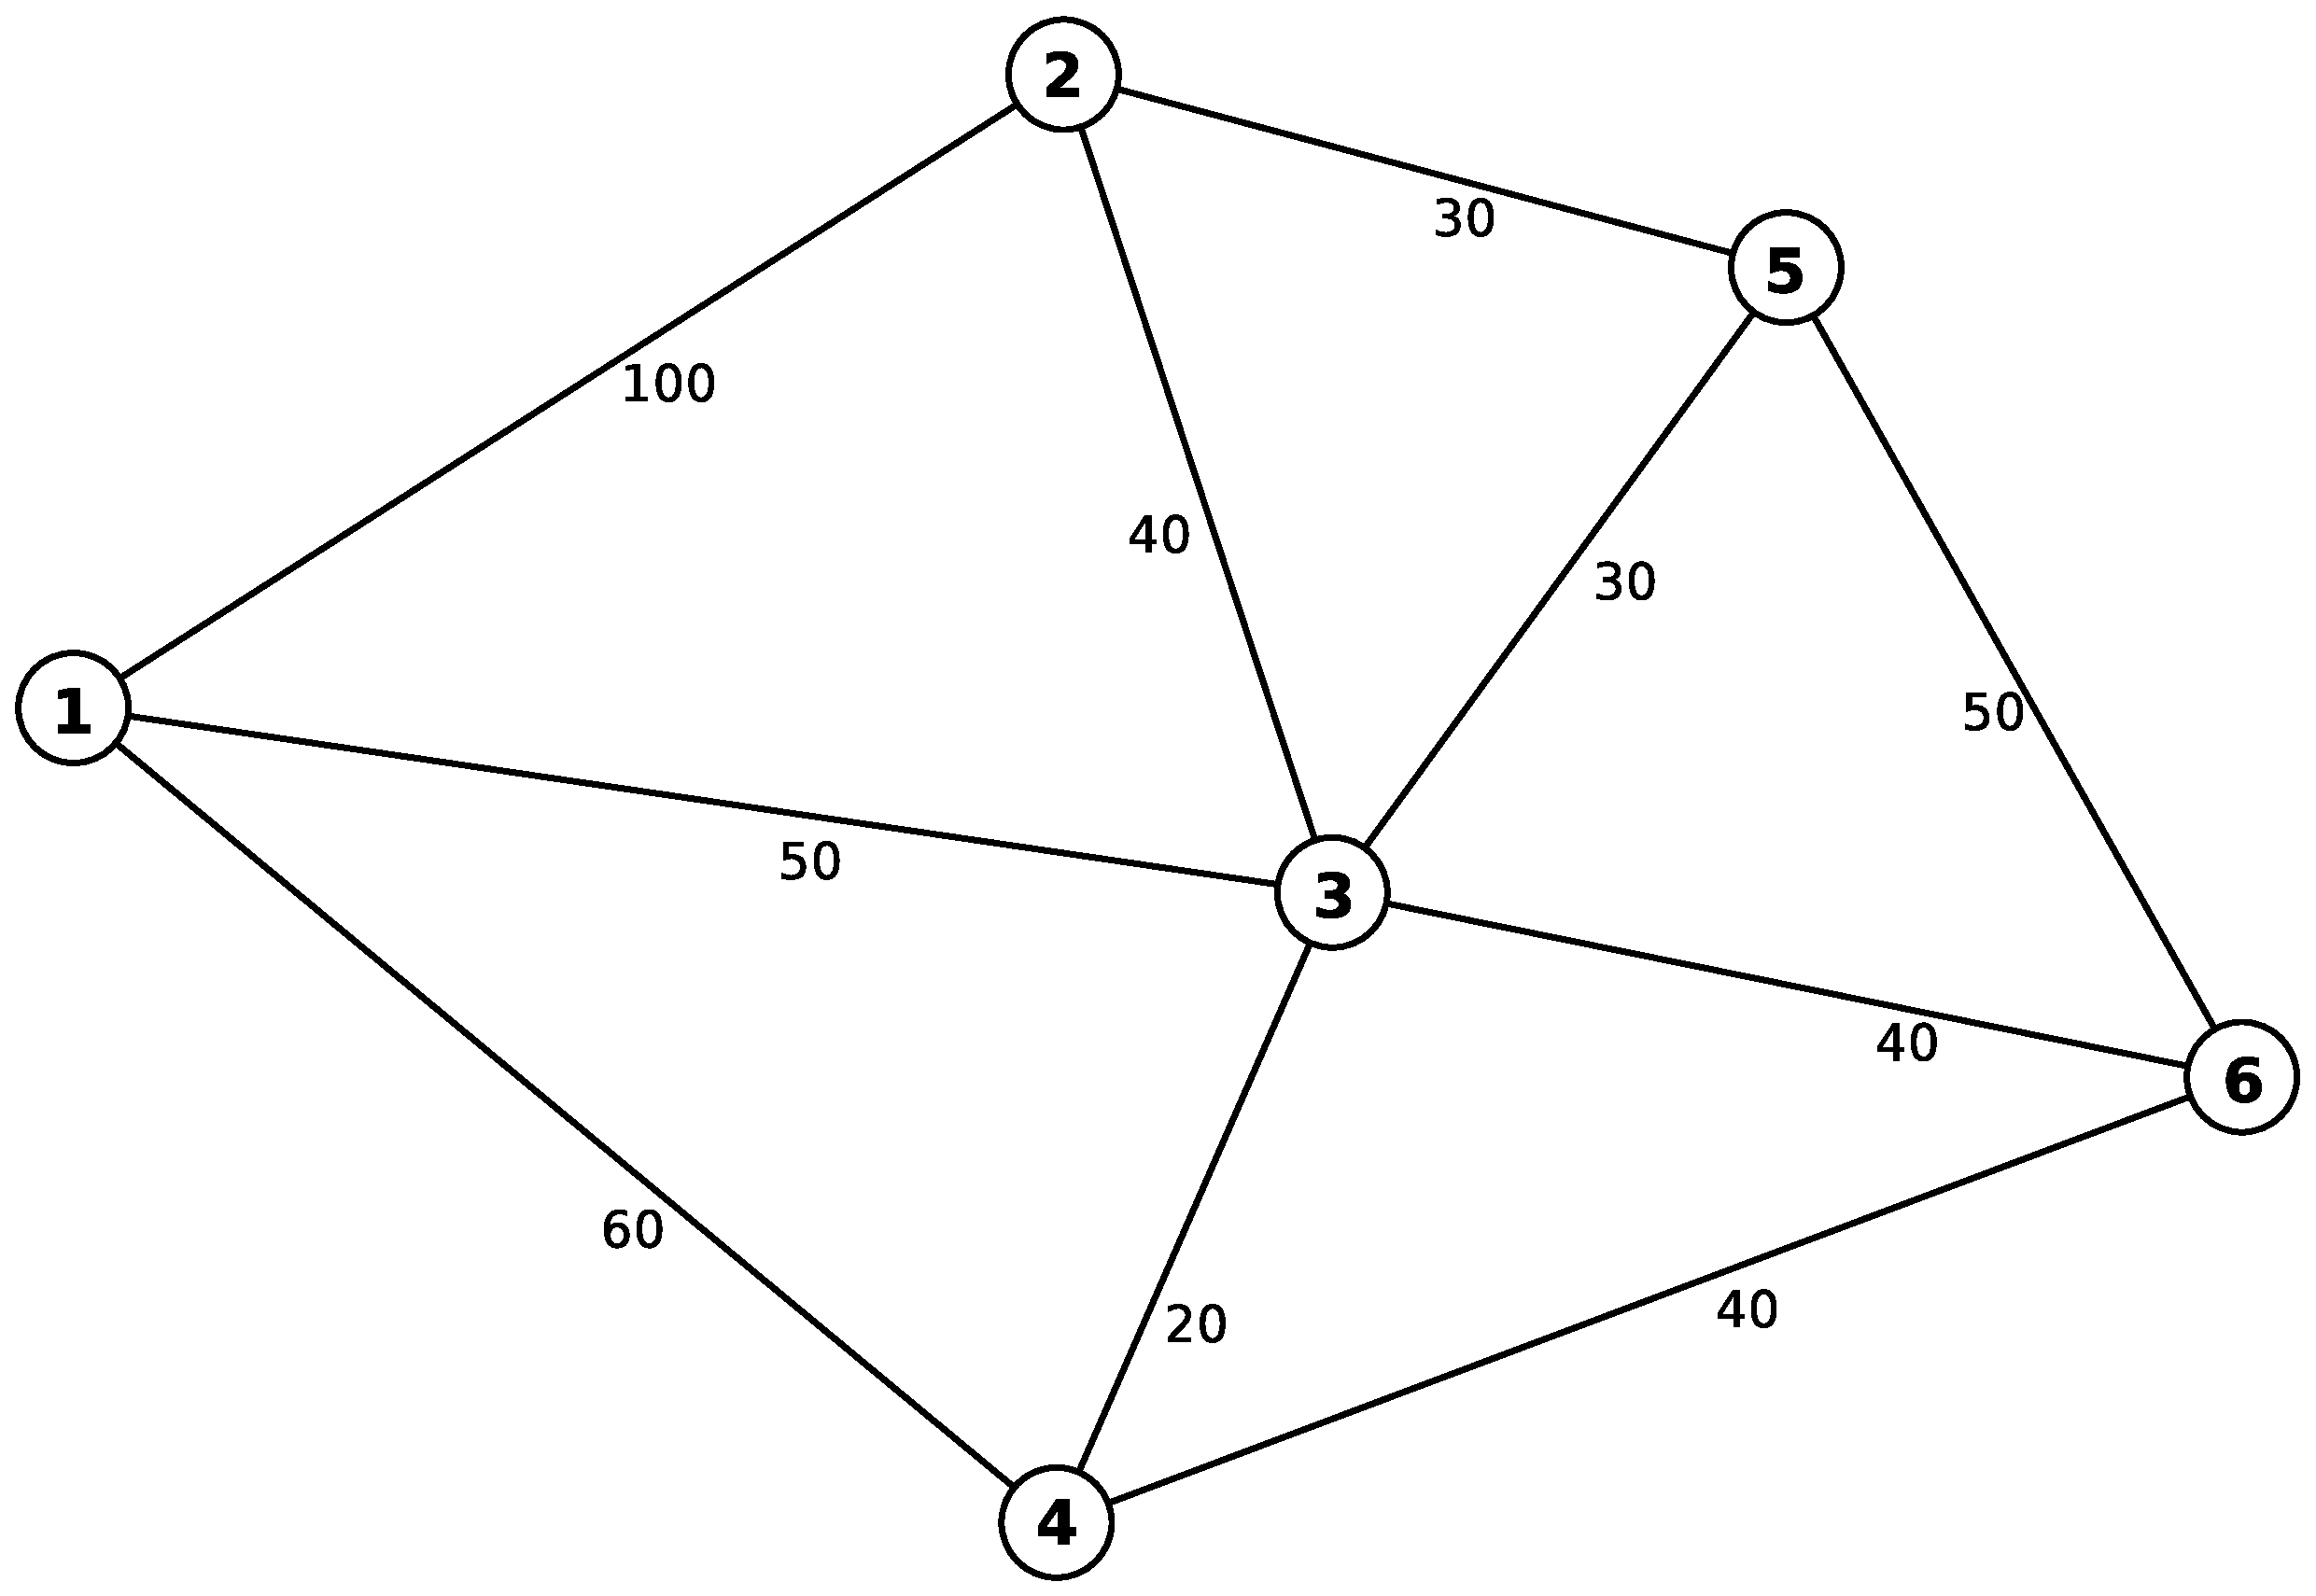
\includegraphics[scale=0.1]{images/figura.eps}
\begin{figure} [h]
\begin {center}
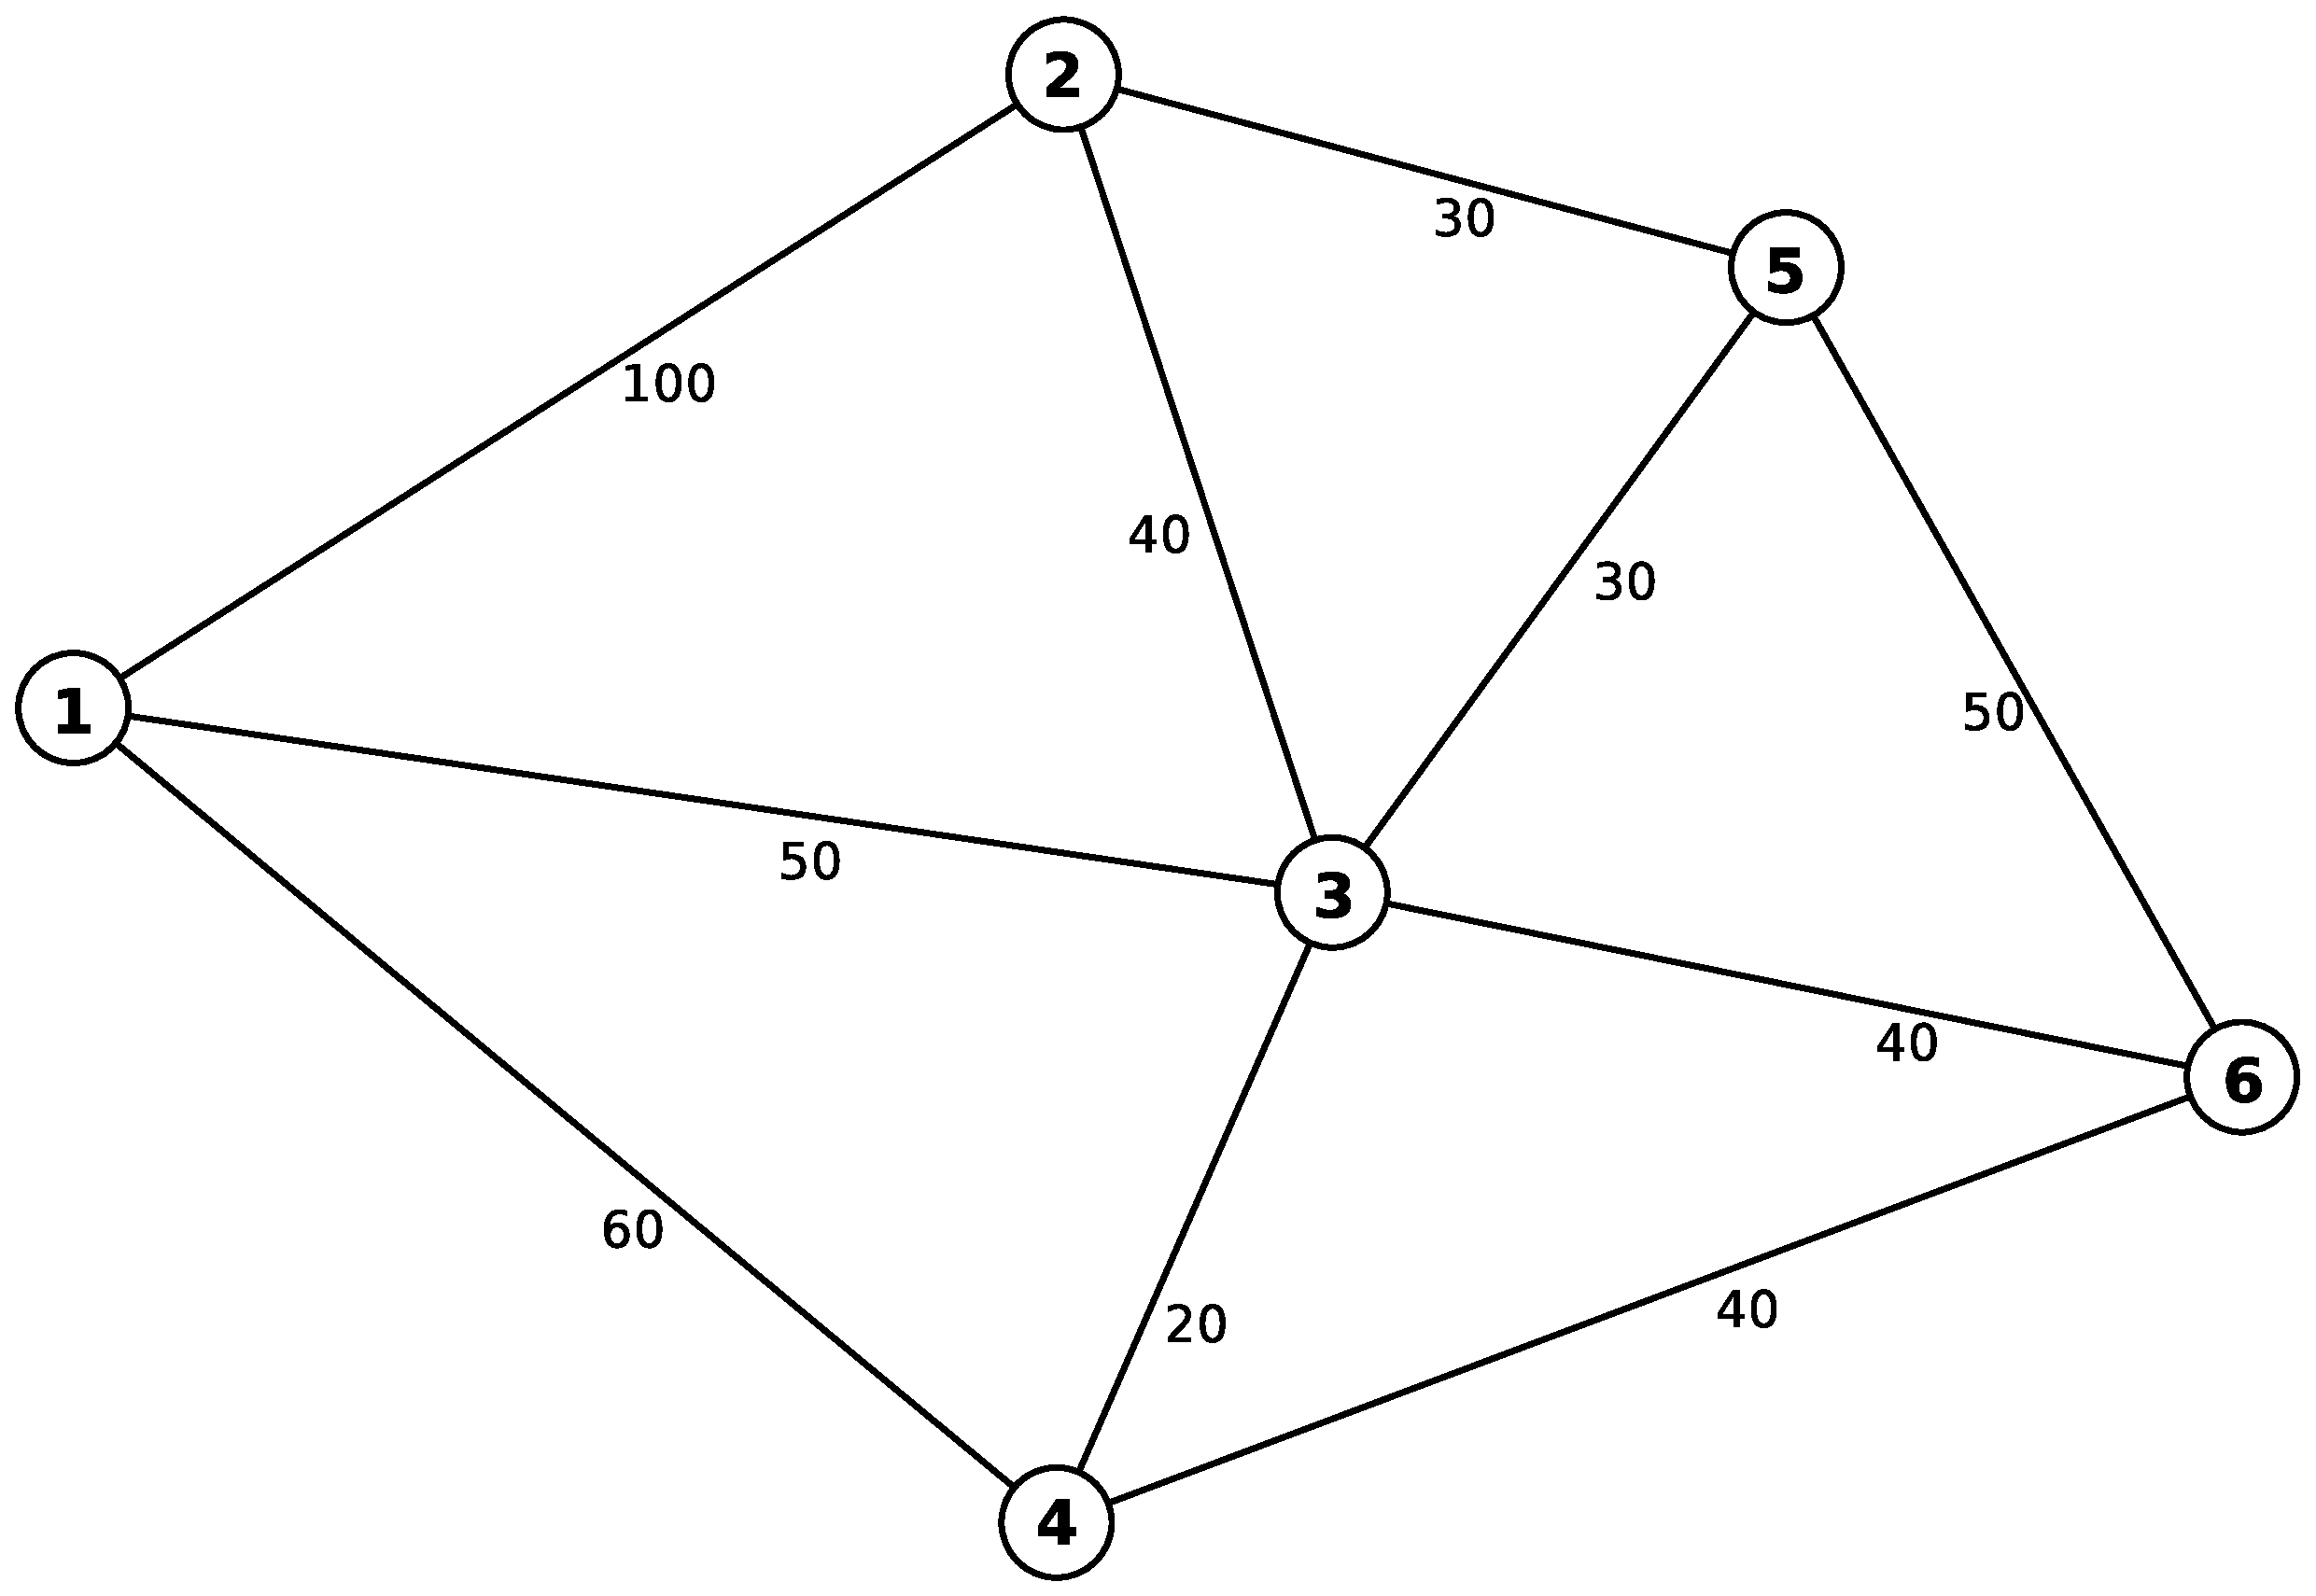
\includegraphics[width=0.8\textwidth]{images/figura.eps}
\end {center}
\end{figure}


En los arcos se definen las capacidades que cada uno de estos puede mantener circulando, en
metros cúbicos por hora.\\

Usando los métodos conocidos responda:\\

1. Determine el flujo máximo que puede entregarse a los generadores. Realice los cálculos de 
\hspace*{0.9cm}forma iterativa y en cada una especifique el flujo acumulado.\\

2. Formule un modelo de programación lineal que le permita satisfacer las restricciones y obtener 
\hspace*{0.9cm}el flujo máximo.\\

3. Realice el mismo trabajo, usando software LINDO o LPSolve. Adjunte sus códigos y comente
\hspace*{0.9cm}sus resultados.\\

\newpage



\bibliographystyle{alpha}
\bibliography{bibbase}

% referencias

\end{document}
